\documentclass[border=1cm]{standalone}

\usepackage{tikz}
\usepackage{medl_colors}

\usetikzlibrary{shapes.geometric, shapes.misc, matrix}
\usetikzlibrary{cd, fit, calc}
\usetikzlibrary{positioning, shadows}
\graphicspath{ {./images/} }

\begin{document}
\begin{tikzpicture}
   \pgfmathsetseed{3}

{\large \matrix (m) [matrix of math nodes, nodes in empty cells, left delimiter=[, right delimiter={]}, row sep=0.3cm, column sep=0.3cm, minimum width=0.4cm, minimum height=0.4cm, scale=0.7] at (3.5, 0) {
        -2.084\\
        0.412\\ 
        -0.84\\
        0.232\\
        -0.424\\
        0.173\\
        0.259\\
        0.985\\
        -1.808\\
        0.112 \\ 
    };
}
    \node[below of= m, node distance=2.4cm, align=center, yshift=-3cm] {\Huge $z$};

    \node[scale=.58] (picd) at (15,-10.5) {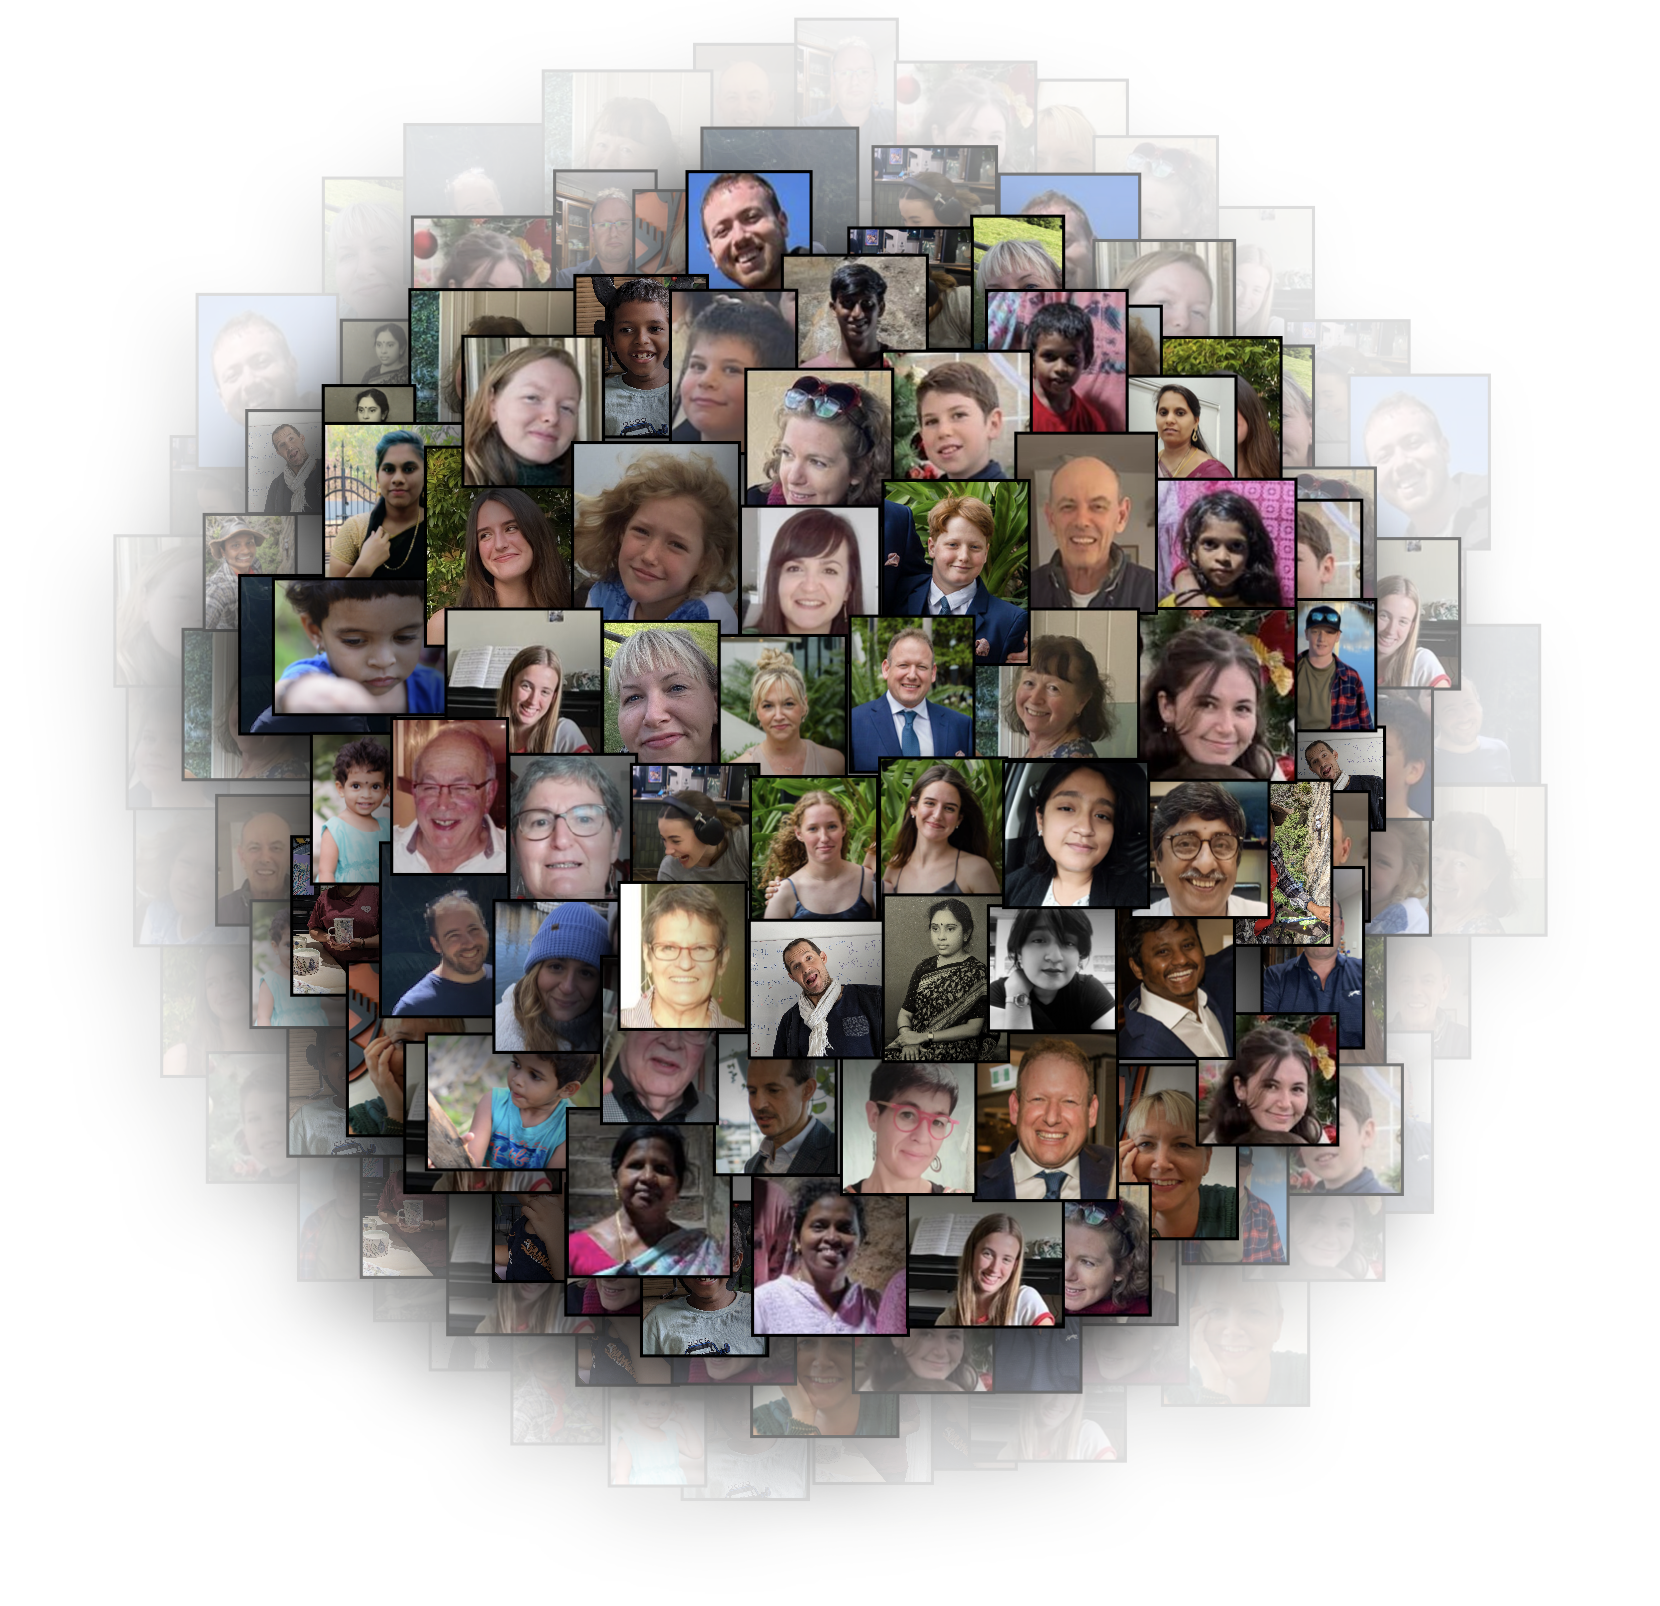
\includegraphics{images/collage.png}};
    
    \node[below right of= picd, node distance=2.4cm, align=center, yshift=-4.2cm, xshift=4.2cm] {\Huge $\mathcal{D}$};
    
    \node[scale=.5, draw, uthickline](picz) at (3.5, -21) {
\includegraphics{images/noisy_image_10.jpg}};
    \node[below of= picz, node distance=2.4cm, align=center] {\Huge $z$};

    \node[blueshape, rounded corners, minimum width=10cm, minimum height=2cm, align=center] (rect1) at (15,0) {\Large GAN Generator \\\,\\ \Large has learned to \textbf{sample} from $p(x | z)$};
    \node[draw, right of= rect1, node distance=11cm, align=center, scale=0.27] (picx1) {
\includegraphics {images/18.png}};
    \node[below of= picx1, node distance=2.4cm, align=center] {\Huge $x$};
    
    \node[blueshape, rounded corners, minimum width=10cm, minimum height=2cm, align=center] (rect2) at (15,-21) {\Large Diffusion Decoder \\\,\\ \Large has \textbf{learned} $p(x | z)$};
    \node[draw, right of= rect2, node distance=11cm, align=center, scale=0.2] (picx2) {
\includegraphics {images/thalli1}};

    \node[below of= picx2, node distance=2.4cm, align=center] {\Huge $x$};
    
    \draw[-Triangle, uthickline] ([xshift=3mm]rect1.east) -- (picx1){};
    \draw[Triangle-, uthickline] ([xshift=-3mm]rect1.west) -- ++(-4, 0){};
    \draw[Triangle-, uthickline] ([yshift=-3mm]rect1.south) -- (picd.north){};
    \draw[-Triangle, uthickline] ([xshift=3mm]rect2.east) -- (picx2){};
    \draw[Triangle-, uthickline] ([xshift=-3mm]rect2.west) -- ++(-4, 0){};
    \draw[Triangle-, uthickline] ([yshift=3mm]rect2.north) -- (picd.south){};
        

\end{tikzpicture}
\end{document}
